% Construction : la courbe de f sur [a, b], avec a = 1 et b = 4,5 ;
% f(x) = 0,45x² − 2,6x + 4,6, positive sur l'intervalle. L'aire hachurée est
% la partie du plan comprise entre l'axe et la courbe.
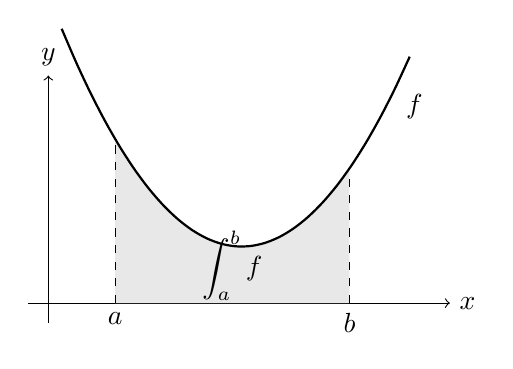
\begin{tikzpicture}[scale=0.85]
  \draw[->] (-0.3, 0) -- (6, 0) node[right] {$x$};
  \draw[->] (0, -0.3) -- (0, 3.4) node[above] {$y$};
  \fill[gray!18, domain=1:4.5, variable=\x]
    (1, 0) -- plot ({\x}, {0.45*\x*\x - 2.6*\x + 4.6}) -- (4.5, 0) -- cycle;
  \draw[thick, domain=0.2:5.4, smooth, variable=\x]
    plot ({\x}, {0.45*\x*\x - 2.6*\x + 4.6});
  \draw[dashed] (1, 0) -- (1, 2.45);
  \draw[dashed] (4.5, 0) -- (4.5, 2.02);
  \node[below] at (1, 0) {$a$};
  \node[below] at (4.5, 0) {$b$};
  \node at (2.75, 0.55) {$\displaystyle\int_a^b f$};
  \node[above right] at (5.2, 2.6) {$f$};
\end{tikzpicture}
